% Options for packages loaded elsewhere
\PassOptionsToPackage{unicode}{hyperref}
\PassOptionsToPackage{hyphens}{url}
%
\documentclass[
]{article}
\usepackage{amsmath,amssymb}
\usepackage{iftex}
\ifPDFTeX
  \usepackage[T1]{fontenc}
  \usepackage[utf8]{inputenc}
  \usepackage{textcomp} % provide euro and other symbols
\else % if luatex or xetex
  \usepackage{unicode-math} % this also loads fontspec
  \defaultfontfeatures{Scale=MatchLowercase}
  \defaultfontfeatures[\rmfamily]{Ligatures=TeX,Scale=1}
\fi
\usepackage{lmodern}
\ifPDFTeX\else
  % xetex/luatex font selection
\fi
% Use upquote if available, for straight quotes in verbatim environments
\IfFileExists{upquote.sty}{\usepackage{upquote}}{}
\IfFileExists{microtype.sty}{% use microtype if available
  \usepackage[]{microtype}
  \UseMicrotypeSet[protrusion]{basicmath} % disable protrusion for tt fonts
}{}
\makeatletter
\@ifundefined{KOMAClassName}{% if non-KOMA class
  \IfFileExists{parskip.sty}{%
    \usepackage{parskip}
  }{% else
    \setlength{\parindent}{0pt}
    \setlength{\parskip}{6pt plus 2pt minus 1pt}}
}{% if KOMA class
  \KOMAoptions{parskip=half}}
\makeatother
\usepackage{xcolor}
\usepackage[margin=1in]{geometry}
\usepackage{graphicx}
\makeatletter
\def\maxwidth{\ifdim\Gin@nat@width>\linewidth\linewidth\else\Gin@nat@width\fi}
\def\maxheight{\ifdim\Gin@nat@height>\textheight\textheight\else\Gin@nat@height\fi}
\makeatother
% Scale images if necessary, so that they will not overflow the page
% margins by default, and it is still possible to overwrite the defaults
% using explicit options in \includegraphics[width, height, ...]{}
\setkeys{Gin}{width=\maxwidth,height=\maxheight,keepaspectratio}
% Set default figure placement to htbp
\makeatletter
\def\fps@figure{htbp}
\makeatother
\setlength{\emergencystretch}{3em} % prevent overfull lines
\providecommand{\tightlist}{%
  \setlength{\itemsep}{0pt}\setlength{\parskip}{0pt}}
\setcounter{secnumdepth}{-\maxdimen} % remove section numbering
\usepackage{ragged2e}
\justifying
\usepackage{titling}
\pretitle{\begin{flushleft}}
\posttitle{\end{flushleft}}
\ifLuaTeX
  \usepackage{selnolig}  % disable illegal ligatures
\fi
\IfFileExists{bookmark.sty}{\usepackage{bookmark}}{\usepackage{hyperref}}
\IfFileExists{xurl.sty}{\usepackage{xurl}}{} % add URL line breaks if available
\urlstyle{same}
\hypersetup{
  pdftitle={Índice Global y Local de Moran en Variación de la Especialización Relativa en Servicios Empresariales e Industria (Papeles de trabajo)},
  pdfauthor={Nicolás Gottig},
  hidelinks,
  pdfcreator={LaTeX via pandoc}}

\title{Índice Global y Local de Moran en Variación de la Especialización
Relativa en Servicios Empresariales e Industria (Papeles de trabajo)}
\author{Nicolás Gottig}
\date{2023-09-22}

\begin{document}
\maketitle

\hypertarget{resumen}{%
\subsection{Resumen}\label{resumen}}

El objetivo es estudiar la especialización relativa relativa en el
sector manufacturero y en el sector de servicios empresariales desde un
enfoque espacial, considerando como unidades los 17 departamentos. Para
esto se calcula la matriz de especialización relativa en 8 ramas
agregadas según el Ministerio de Obras Públicas, se estudia su evolución
y se identifica que Islas del Ibicuy presenta valores atípicos en la
especialización relativa del sector servicios, así como un marcado
comportamiento a priori, cíclico y estacionario. Por lo tanto, se
excluye del análisis final. Por otro lado, se estudia la asociación
entre la especialización relativa, permitiendo clasificar a los
departamentos en especializados en manufactura, especializados en el
sector primario o especializados en enseñanza y salud. Por último, se
estudia la autocorrelación espacial a través del Índice Global de Morán,
y se analiza la presencia de aglomerados de especialización a través del
Índice Local de Moran, concluyendo en que la especialización relativa de
los sectores industriales y de servicios empresariales se distribuyen de
forma azarosa en la provincia, y no existe una tendencia al agrupamiento
espacial ni un ``derrame'' entre vecinos.

\hypertarget{anuxe1lisis-de-matriz-de-especializaciuxf3n-relativa}{%
\subsection{Análisis de matriz de especialización
relativa}\label{anuxe1lisis-de-matriz-de-especializaciuxf3n-relativa}}

Los datos para el cálculo de la matriz se encuentran en el archivo
``matriz-especializacion-complleta.txt''. Dicho archivo contiene, para
cada año, el cálculo de la especialización relativa por departamento y
rama agregada según criterio del MOP. A partir de esto, se desea
estudiar la evolución de la especialización relativa en el sector
manufacturero y en el sector de servicios empresariales por año:

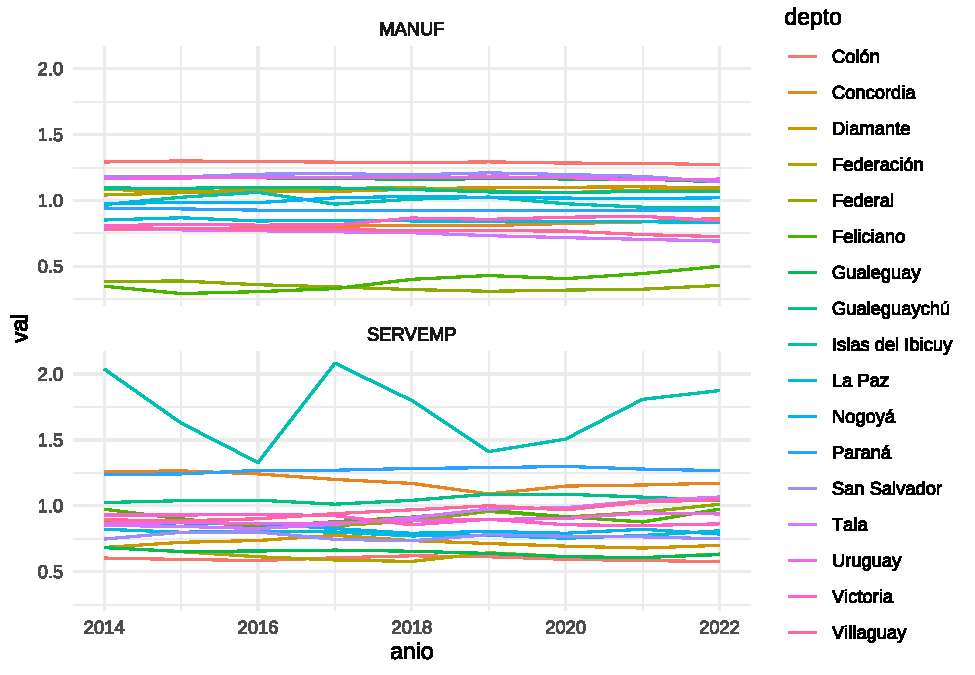
\includegraphics{documento-final_files/figure-latex/unnamed-chunk-1-1.pdf}
Se observa que Islas del Ibicuy presenta un comportamiento estable en la
especialización de la industria manufacturera, pero presenta grandes
oscilaciones en la industria de servicios empresariales; casi
duplicando, en ciertos años, su participación relativa en el sector. Por
lo tanto, se decide excluirla del análisis posterior y estudiarla de
forma individual. Sin este departamento, la evolución de los sectores en
cada departamento se da de la siguiente forma:

\begin{figure}
\centering
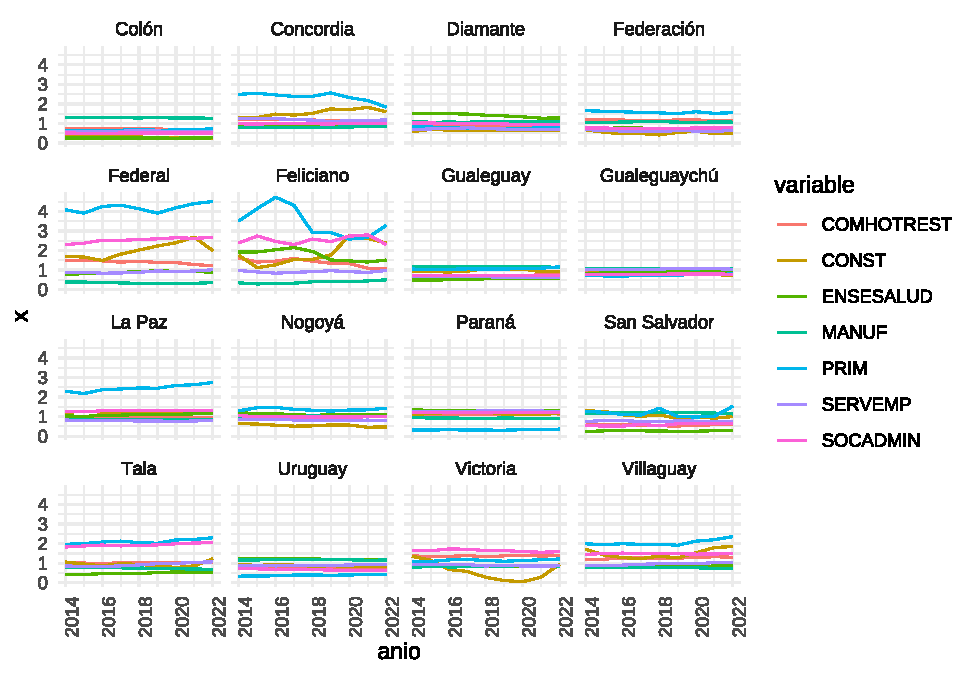
\includegraphics{documento-final_files/figure-latex/unnamed-chunk-2-1.pdf}
\caption{Esp. Relativa por departamento y serctor sin Islas del Ibicuy}
\end{figure}

Se destaca una disminución de la especialización relativa en el sector
primario en Concordia desde el 2019, en contraposición a un aumento en
la esp.~Relativa del sector de construcción. En el caso de Federal y
Feliciano, sobresalen en términos de especialización relativa en el
sector primario, y de servicios sociales y administración pública frente
al resto.\\
También se identifican comportamientos sobresalientes en algunos
sectores en La Paz, Rosario del Tala y Villaguay. ASí como un cambio de
tendencia en el sector de construcción en victoria, con una tendencia
creciente desde 2020.

Sin Islas del ibicuy, la tasa de variación entre el 2022 y el 2014 de la
especialización relativa en la provincia queda de la siguiente manera:

\begin{verbatim}
## [1] "en_US.UTF-8"
\end{verbatim}

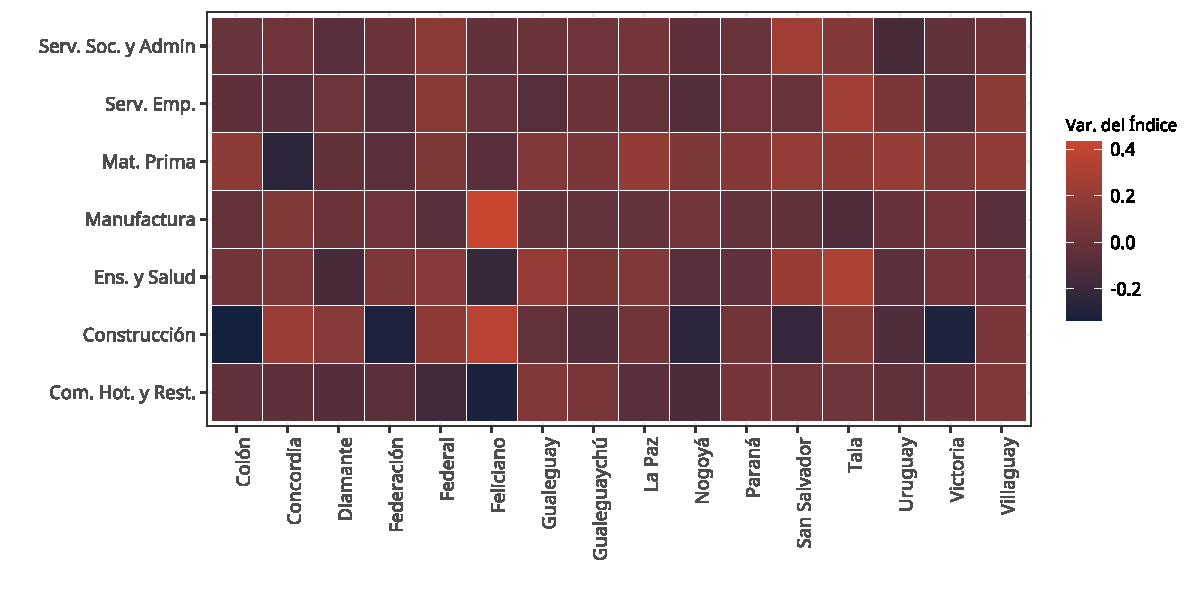
\includegraphics{documento-final_files/figure-latex/unnamed-chunk-3-1.pdf}
\#\# Caracterización de los perfiles productivos en las provincias según
especialización relativa

Para la caracterización de las unidades bajo estudio se utilizan
proyecciones multivariadas en las variables que recogen la
especialización de un sector en cada unidad. Las dos primeras
proyecciones explican casi el 80 \% de la variabilidad total, por lo que
se utilizarán sólo esos para el análisis.

\end{document}
